\documentclass[11pt,letterpaper]{article}
\usepackage[T1]{fontenc}
\usepackage{lmodern,amsmath,amssymb,booktabs,tabularx,graphicx,microtype}
\usepackage[margin=0.8in]{geometry}
\usepackage[colorlinks=true,urlcolor=blue!60!black,linkcolor=blue!60!black]{hyperref}
\usepackage{xcolor}
\setlength{\emergencystretch}{3em}
\setlength{\parskip}{0.3em}
\newcommand{\pc}{P^{\mathrm c}}
\title{Pair correlations survive locally in stripe states\\
\large Complete retrospective measurements and square A/B results}
\author{Ladder MPS+MF project}
\date{22 September 2026}
\begin{document}
\maketitle

\noindent\textbf{Main result.}
Stripe formation does not eliminate short-distance singlet-pair correlations.
In the representative square, cubic and trellis stripe snapshots, these
correlations concentrate near hole-rich magnetic domain walls, while propagation
over 16--24 rungs is strongly suppressed. Rung--leg correlations retain a
predominantly negative relative sign. This separates local pairing from
long-distance order, but does not establish fluctuating superconductivity,
phase stiffness or a dynamical phase-disordering mechanism.

\noindent\textbf{New square result.}
All four square two-ladder runs at $t_0=1.4$ and $V=-0.4,-0.2$ pass the
stored fixed-point gates. Both seeds approach nearly identical paired A/B
profiles and pair correlations at each $V$, despite the displaced stripe
component in the initial conditions. This supports survival of the paired
solution in the tested square cell. It does not establish stability against
arbitrary transverse periods or a global minimum.

\section{Coverage and operator convention}
The synchronized retrospective campaign now covers all 56 branches and
58 spatial MPSs: 49 receipts/51 MPSs in retry1 and seven receipts/MPSs in
retry2. The new square A/B campaign supplies eight further diagnostics from
four accepted branches. The isolated reference is the earlier $L=64$,
$t_0=1.4,V=0$, $\chi=1200$ backbone. All coupled measurements use $\chi=200$,
$U=8$, $n=15/16$, and $L=64$ rungs per MPS. Retrospective endpoints remain
\emph{unaccepted maximum-iteration snapshots}; completing measurements does
not change their scientific convergence status. Trellis A/B labels are
spatial ladders, not temporal cycle phases.

Use the stored, unnormalized bond singlet
\begin{equation}
 D_{ab}=c_{a\uparrow}c_{b\downarrow}-c_{a\downarrow}c_{b\uparrow},\qquad
 P_{ab,cd}=\langle D_{ab}^{\dagger}D_{cd}\rangle,\qquad
 \pc_{ab,cd}=P_{ab,cd}-\langle D_{ab}\rangle^*\langle D_{cd}\rangle.
\end{equation}
The manuscript's normalized singlet is $\Delta=D/\sqrt2$; its correlations
are one half of the values here. Stored onsite operators are instead
$c_\uparrow c_\downarrow$. The 318-coordinate basis comprises 64 rung,
126 nearest-neighbor leg and 128 onsite operators. Rung--leg separation is
defined by the start rung, so bond midpoints differ by half a rung.

The older isolated-ladder file stores within-class Hermitian-field covariances,
with non-onsite operators divided by $\sqrt2$. On this real,
number-conserving reference and for \emph{disjoint} bonds, that covariance
equals $\operatorname{Re}\langle D_i^\dagger D_j\rangle$:
$(\langle D_iD_j^\dagger\rangle+\langle D_i^\dagger D_j\rangle)/2$.
The anomalous expectation is zero. Contact rung entries and overlapping
leg entries are excluded. Rung--leg cross-channel data are unavailable for
this older reference and are not reconstructed. Its larger bond dimension
precludes a controlled attribution of all differences to transverse coupling.

\section{Short-distance survival and long-distance suppression}
Distance curves average $|P_{ij}|$ or $|\pc_{ij}|$ over both orientations
with rung bonds in rungs 9--56 and leg-bond starts in 9--55, so both endpoints
remain in that bulk window. The signed averages and their spatial 10th/90th percentiles are
saved separately. Spatial spread is not a statistical confidence interval.
Table~\ref{tab:strength} averages the entries in two separation bands;
different separations carry the number of available bulk pairs.

\begin{table}[htbp]\centering\small
\caption{Rung-pair magnitudes in the common stored convention. Representative
paired-seed endpoints; trellis two-ladder entry is A. All coupled rows in this
table are unaccepted snapshots. $S$ and $L$ denote separations 2--4 and 16--24.}
\label{tab:strength}
\begin{tabular}{lrrr}\toprule
State $(t_0,V)$ & $\overline{|\pc|}_S$ & $\overline{|\pc|}_L$ & $\overline{|P|}_L$\\\midrule
Isolated $(1.4,0)$, $\chi=1200$ & $2.0345\,10^{-2}$ & $5.2195\,10^{-3}$ & $5.2195\,10^{-3}$\\
Square paired $(1.4,-0.4)$ & $1.1816\,10^{-2}$ & $3.0361\,10^{-4}$ & $1.1661\,10^{-2}$\\
Square stripe $(1.4,0)$ & $1.5090\,10^{-2}$ & $9.8143\,10^{-5}$ & $9.8143\,10^{-5}$\\
Cubic stripe $(1.4,-0.4)$ & $1.0064\,10^{-2}$ & $1.2935\,10^{-7}$ & $1.2935\,10^{-7}$\\
Trellis one-ladder paired $(1,0)$ & $5.9777\,10^{-3}$ & $4.6411\,10^{-5}$ & $4.3956\,10^{-3}$\\
Trellis two-ladder stripe $(1,0)$ & $5.8648\,10^{-3}$ & $6.6518\,10^{-7}$ & $6.6518\,10^{-7}$\\\bottomrule
\end{tabular}
\end{table}

The square $V=0$ stripe retains roughly 74\% of the isolated reference's
short-distance magnitude but only 1.9\% of its long-distance magnitude.
The latter is a descriptive comparison across $\chi=200$ and 1200, not a
bond-dimension-controlled suppression factor. Both square stripe seeds give
the same qualitative result ($8.19$--$9.81\,10^{-5}$ at long distance).

Comparisons at matched intraladder parameters are sharper. Square paired
and cubic striped snapshots at $(1.4,-0.4)$ have comparable short-distance
connected magnitudes, while the cubic long-distance value is about
$2.2$--$2.3\,10^3$ smaller. For trellis at $(1,0)$, the one-/two-ladder
short-distance values differ by only a few percent, whereas the striped
two-ladder long-distance connected value is about 70 times smaller.
These are differences between saved endpoints and spatial embeddings,
not a controlled causal intervention or a stationary phase ranking.

In the square paired state, approximately 97.4\% of the long-distance
\emph{signed} full rung correlation is the disconnected product of anomalous
expectations. The corresponding raw/connected curves are essentially
identical in the representative stripes. Thus an ordered-state plateau
and the decay of residual pair fluctuations answer different questions.

\begin{figure}[p]\centering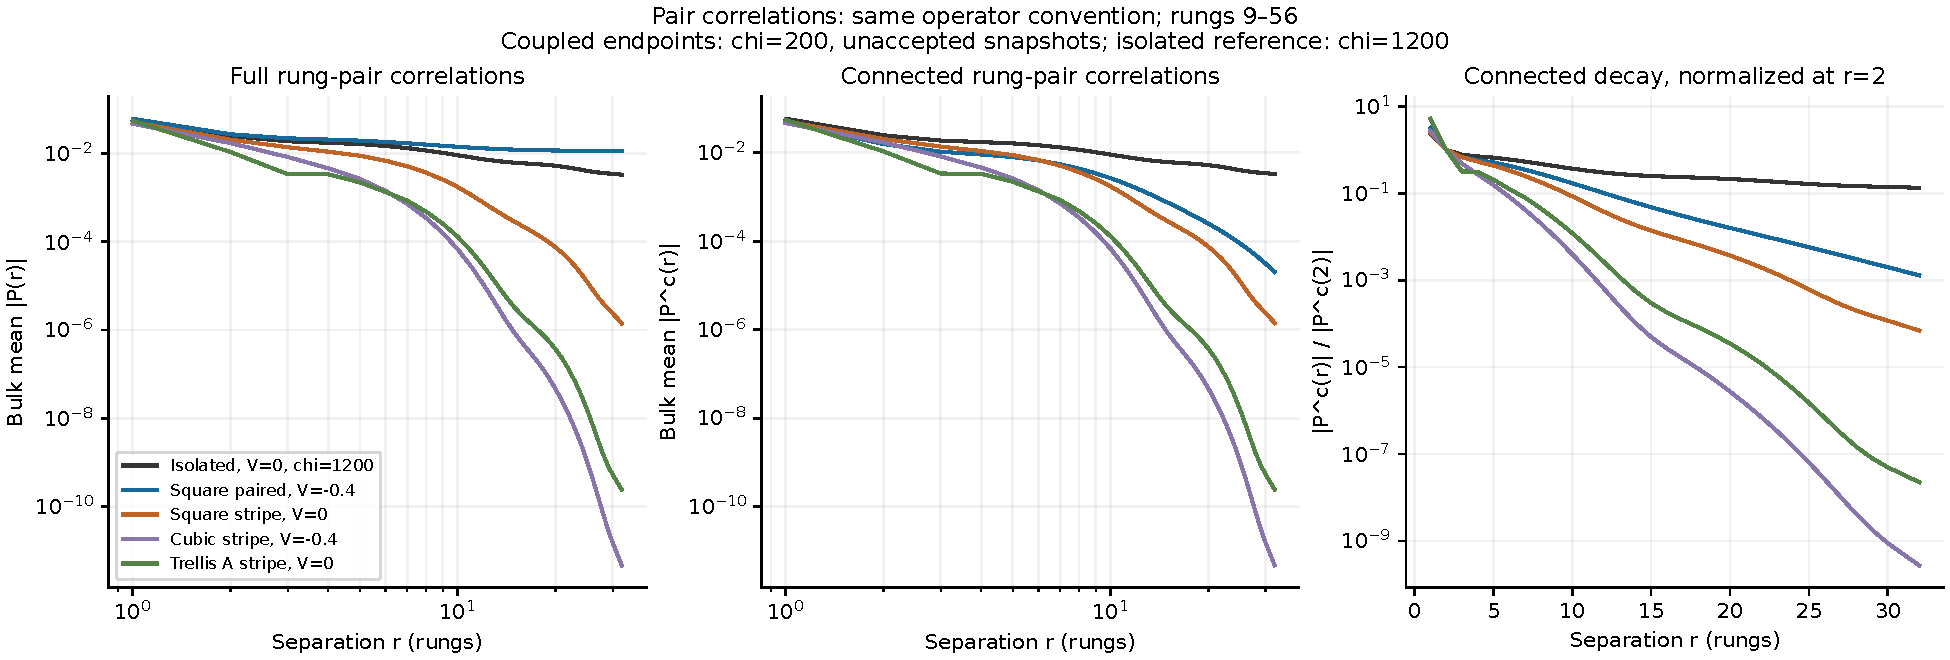
\includegraphics[width=\textwidth]{pair_decay_comparison.pdf}
\caption{Full, connected and normalized connected rung-pair correlations.
The trellis curve has $t_0=1,V=0$; the other four have $t_0=1.4$.
Magnitudes retain oscillatory contributions rather than cancelling signs.
The farthest, very small tails have no independent truncation-error estimate.}
\end{figure}
\begin{figure}[p]\centering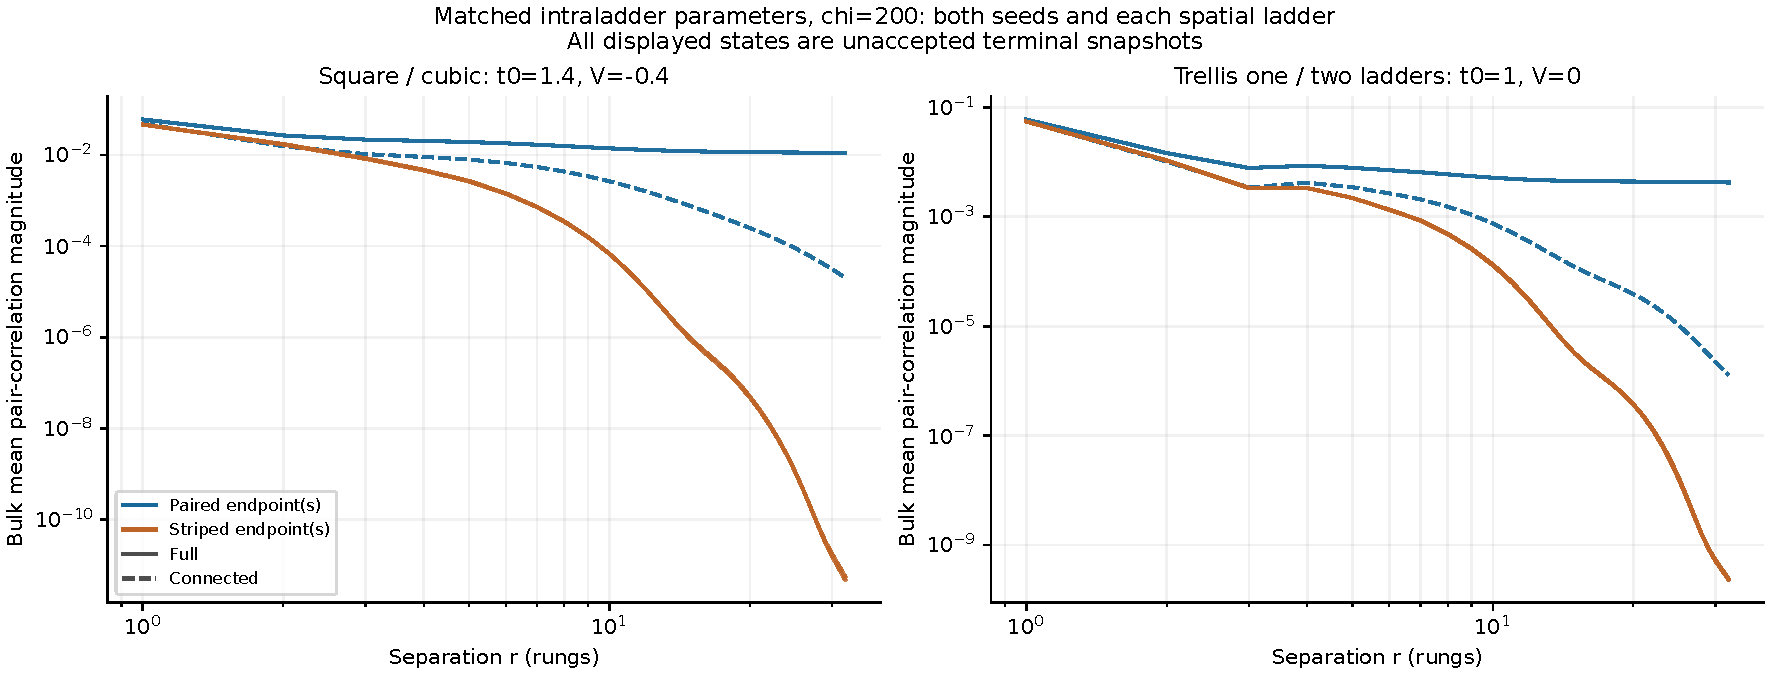
\includegraphics[width=\textwidth]{matched_pair_comparisons.pdf}
\caption{Matched intraladder-parameter comparisons including both initial
families and, where present, both spatial ladders. Solid/dashed lines separate
full and connected values. Similar short-distance amplitudes coexist with
strongly different long-distance behavior.}
\end{figure}
\clearpage

\section{Bond signs and location within stripes}
For the representative square paired, square striped and cubic striped
states, rung--rung and leg--leg averages are positive while rung--leg
averages are negative. Over separations 2--8 in the bulk, the selected
square stripe gives leg--leg $4.31\,10^{-3}$ and rung--leg
$-7.07\,10^{-3}$; the cubic stripe gives $1.90\,10^{-3}$ and
$-3.66\,10^{-3}$, respectively. These are connected values.
Across all 58 retrospective MPSs, the negative fraction of connected
rung--leg0 entries in this band is 96.3--100\% on square, 87.2--100\% on
cubic and 100\% on trellis. Leg1 is retained separately in the data table.
This is compatible with a local rung/leg sign structure commonly called
$d$-wave-like, not proof of a condensate or pair-density wave.

The trellis case also warns against an overly uniform form-factor claim:
its leg--leg correlations change sign with separation. In the two-ladder
striped example, the signed leg0 mean over 2--8 is about $-4.1\,10^{-5}$
even though the nearest values are positive and rung--leg entries remain
negative. The signed channel plots and tables should accompany magnitude
plots whenever internal pair structure is discussed.

Define a local diagnostic
\begin{equation}
 A(i)=\frac16\sum_{r=2}^{4}
 \bigl(|\pc_{\rm rung}(i,i+r)|+|\pc_{\rm rung}(i,i-r)|\bigr).
\end{equation}
Use centers 13--52, so all six neighbors lie in the common bulk window.
Compare the ten centers in the highest hole-density quartile with the ten in
the lowest; no fitting or peak tuning is needed for this amplitude ratio.
The ratio is 5.85--6.68 for the two square $V=0$ seeds, 19.39--19.59 for
the two cubic $(1.4,-0.4)$ seeds, and 5.29--5.36 over both seeds/ladders
of striped trellis. Interior hole-density maxima lie within half a rung
of the discrete staggered-spin sign crossings. The strongest short-distance
pair correlations therefore sit near hole-rich antiphase walls.
Spatial observations in a single texture are correlated; these ratios are
descriptive and do not establish a mechanism of stripe-induced attraction.

\begin{figure}[p]\centering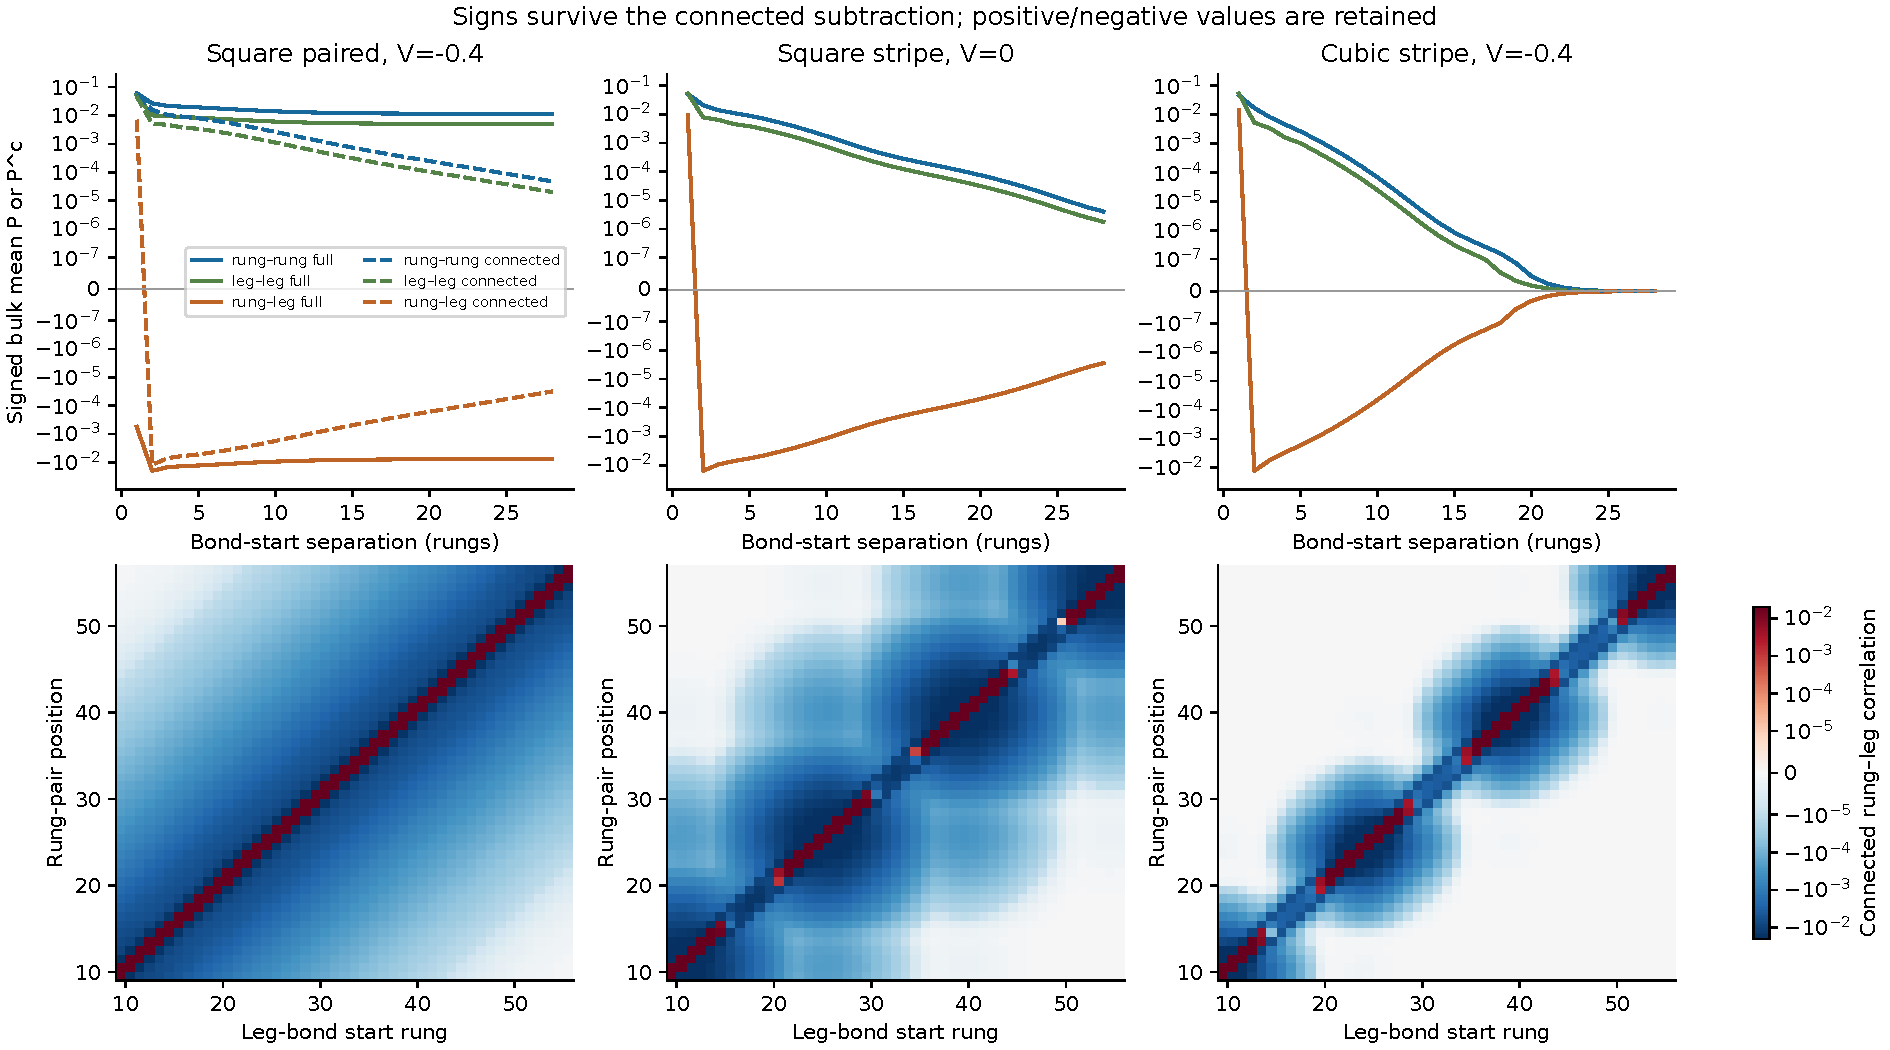
\includegraphics[width=\textwidth]{pair_channel_signs.pdf}
\caption{Signed full/connected rung--rung, leg0--leg0 and rung--leg0 curves,
with connected rung--leg maps below. Symmetric-log scales preserve sign and
small values; matrix contact regions should not be interpreted as propagation.
The isolated reference lacks cross-channel measurements.}
\end{figure}
\begin{figure}[p]\centering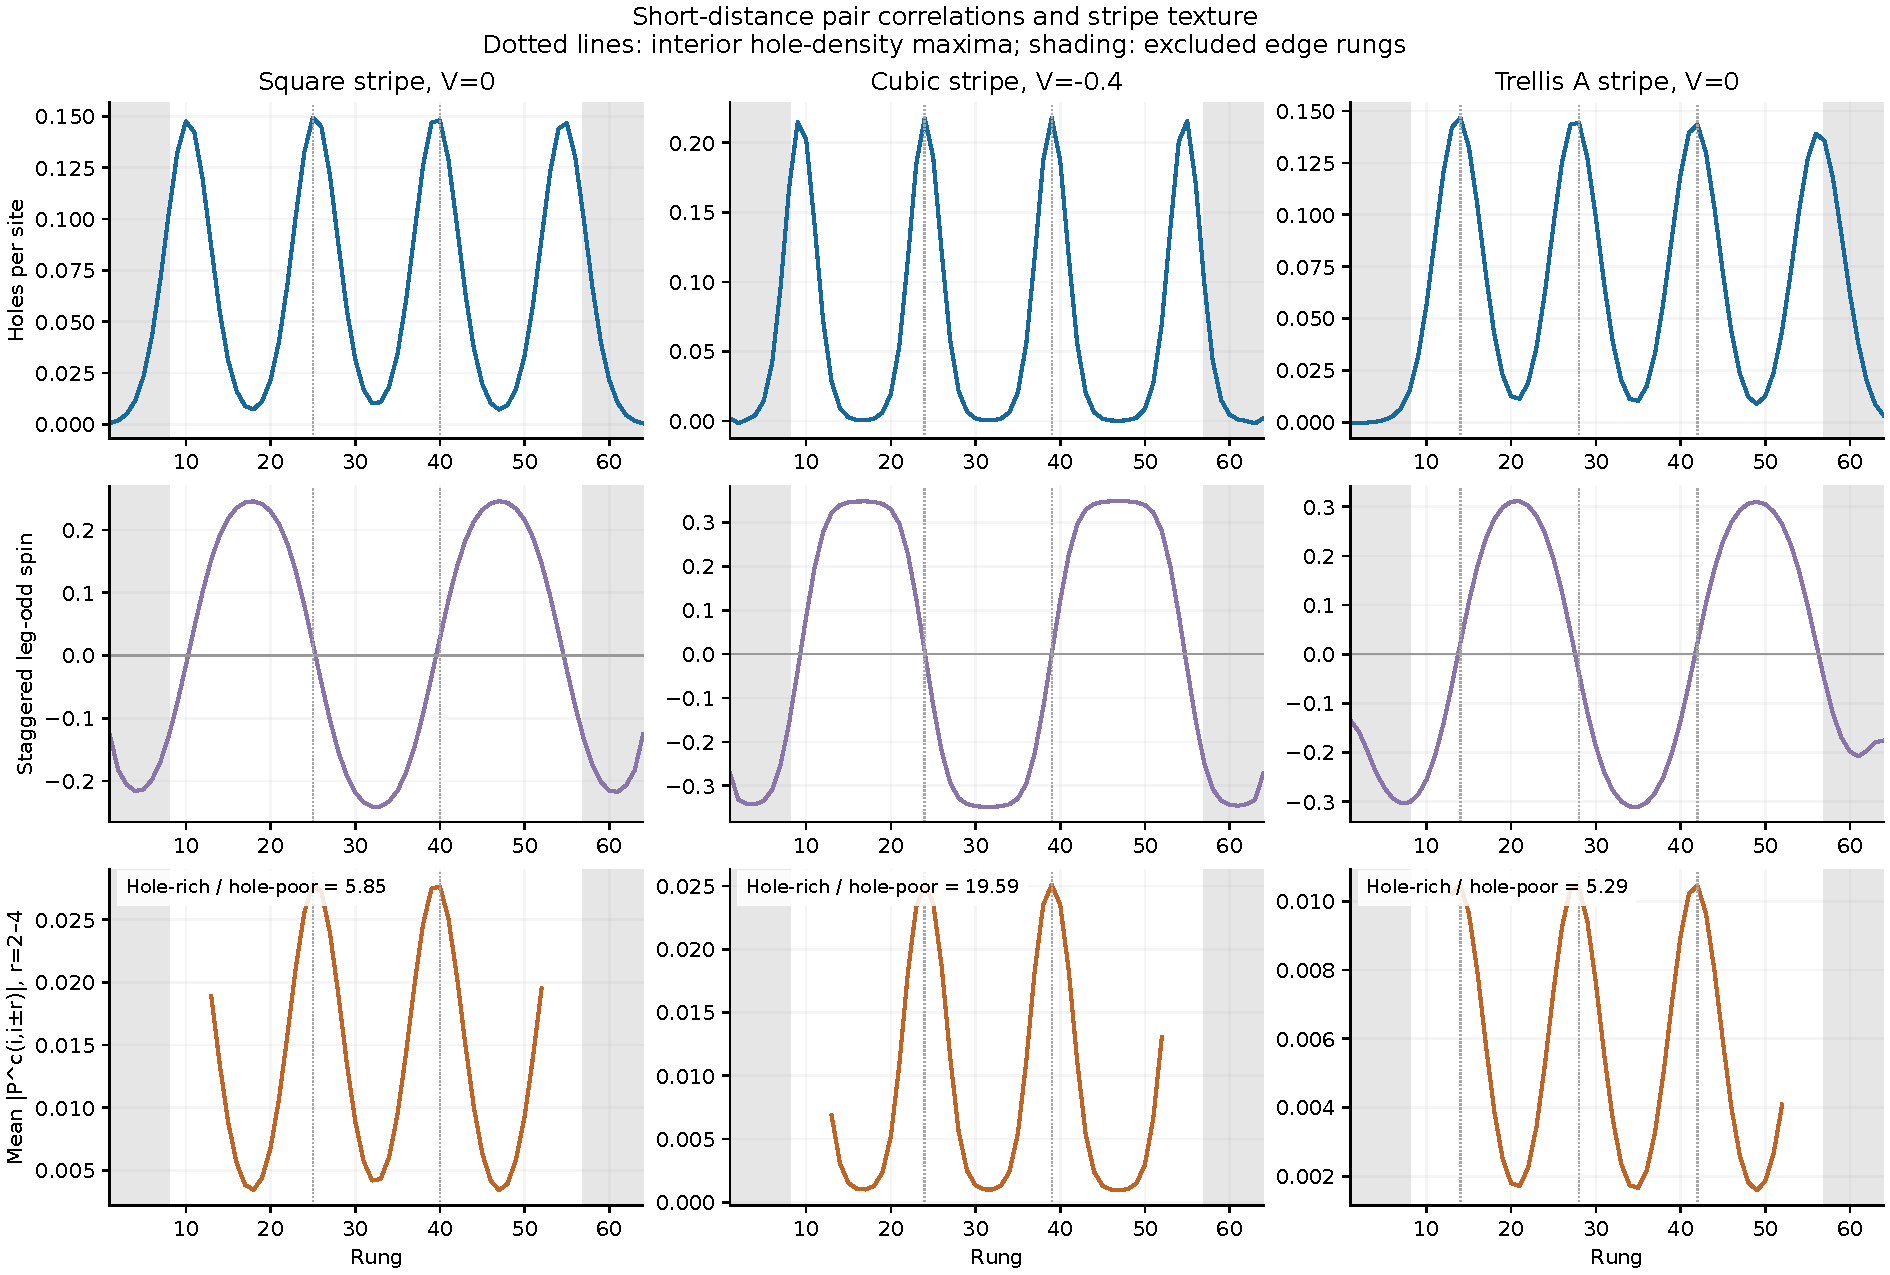
\includegraphics[width=\textwidth]{stripe_pairing_profiles.pdf}
\caption{Hole density, staggered leg-odd spin and local pair diagnostic $A(i)$.
Shading excludes the outer eight rungs; $A(i)$ uses the stricter center
window 13--52. Dotted lines identify interior hole maxima. The three columns
are representative snapshots, not three independent statistical ensembles.}
\end{figure}
\clearpage

\section{Reference, window and boundary sensitivity}
We fit $\log|\pc(i,i\pm r)|$ separately for reference rungs 16, 24 and 32,
both directions, and windows 4--12, 8--20 and 12--28. Windows are clipped
to endpoints inside rungs 9--56; fits need at least six points above
$10^{-12}$. Actual ranges and sign changes are saved. The threshold is
an analysis filter, not a validated numerical accuracy bound. Power and
exponential fits use the same points and two fitted parameters; their
log residual RMS is only a descriptive comparison.

For the isolated rung reference the effective power slopes span 0.39--1.36,
broader than the previously reported window-averaged fit near 0.76. The
square paired \emph{connected} slopes span 1.55--4.12, square stripe
$-0.50$--6.74, cubic stripe 0.37--15.55, and trellis stripe 1.92--13.64
for the displayed representatives. Negative effective slopes arise from
fitting across spatial modulations. No common asymptotic exponent follows
from these ranges. In particular, subtracting a paired-state plateau changes
the function being fit.

This check follows the boundary concern demonstrated by Shen, Zhang and Qin,
\href{https://doi.org/10.1103/PhysRevB.108.165113}{Phys. Rev. B 108, 165113 (2023)}:
reference-bond selection can strongly affect extracted pair exponents.
The source is used for the methodological motivation, not as a numerical
benchmark for this extended, mean-field-coupled Hamiltonian.
The supplied bulk-cut table additionally excludes 4, 8 or 12 rungs at each
end. The representative square stripe's long-distance magnitude remains
$8.99$--$10.31\,10^{-5}$, cubic $1.15$--$1.39\,10^{-7}$ and trellis
$6.19$--$6.97\,10^{-7}$ across those cuts. The finite-distance ordering
survives this change, unlike any universal fitted-exponent claim.
Independent larger-$L$/$\chi$ results remain necessary.

\begin{figure}[htbp]\centering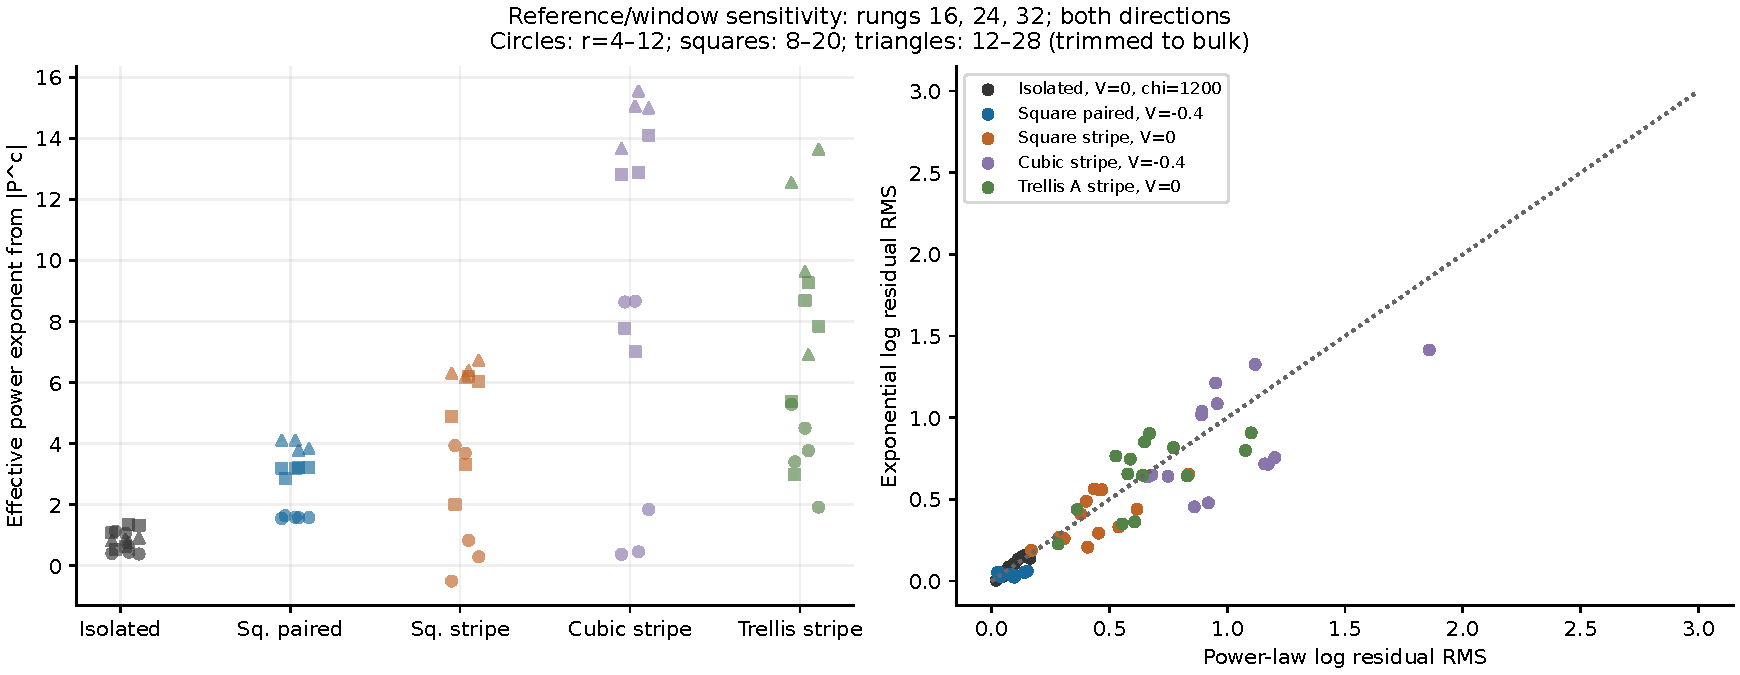
\includegraphics[width=\textwidth]{reference_window_sensitivity.pdf}
\caption{Fit sensitivity, not confidence intervals. The right panel compares
two descriptive decay forms on identical observations. Neither a favorable
$R^2$ nor a smaller residual certifies an asymptotic power law or exponential.}
\end{figure}
\clearpage

\section{Completed square A/B campaign}
All four runs at $t_0=1.4$ reach accepted fixed points. The analysis checks
source/configuration/seed hashes, raw-update identities, final ten-step
channel and density gates, inner-DMRG energy changes, slow-mode criteria,
energy windows and Hamiltonian consistency. It also reconstructs canonical
energies and their target-density correction with 256 physical sites per cell.

\begin{table}[htbp]\centering
\caption{Completed square A/B endpoints. Pair RMS is the historical physical
symmetrized leg anomalous expectation on bonds 6--58, not $D$ or a pair--pair
correlator. The two seed energies agree; they are not distinct energy-ranked phases.}
\begin{tabular}{rrlrr}\toprule
$V$ & Sweeps & Seed & $E_{\rm target}/(Nt)$ & Leg-pair RMS\\\midrule
$-0.4$ & 40 & Stripe & $-1.167404800596$ & $0.0352251$\\
$-0.4$ & 40 & Pairing & $-1.167404800545$ & $0.0352251$\\
$-0.2$ & 55 & Stripe & $-0.914117842951$ & $0.0335678$\\
$-0.2$ & 44 & Pairing & $-0.914117843004$ & $0.0335678$\\\bottomrule
\end{tabular}
\end{table}

Within a fixed $V$, the seed energy difference is at most
$5.3\,10^{-11}\,t$/site. Final bulk spin RMS is below $5.4\,10^{-7}$ at
$V=-0.4$ and below $1.15\,10^{-6}$ at $V=-0.2$. Maximum A/B differences
in physical leg-pair profiles are below $1.1\,10^{-6}$; residual charge
differences reach $1.13\,10^{-5}$. The stripe displacement in the initial
condition does not survive as a distinct stationary magnetic texture.

Connected long-distance rung-pair magnitudes are about $3.036\,10^{-4}$
at $V=-0.4$ and $2.475\,10^{-4}$ at $V=-0.2$, with nearly overlapping
curves from both seeds and ladders. Full magnitudes remain about
$1.166\,10^{-2}$ and $1.030\,10^{-2}$. The new cell reproduces the paired
one-ladder snapshots' correlations as well as their anomalous profiles.
All measurements are \emph{intraladder}; the mean-field spatial extension
does not introduce interladder quantum entanglement.

\begin{figure}[p]\centering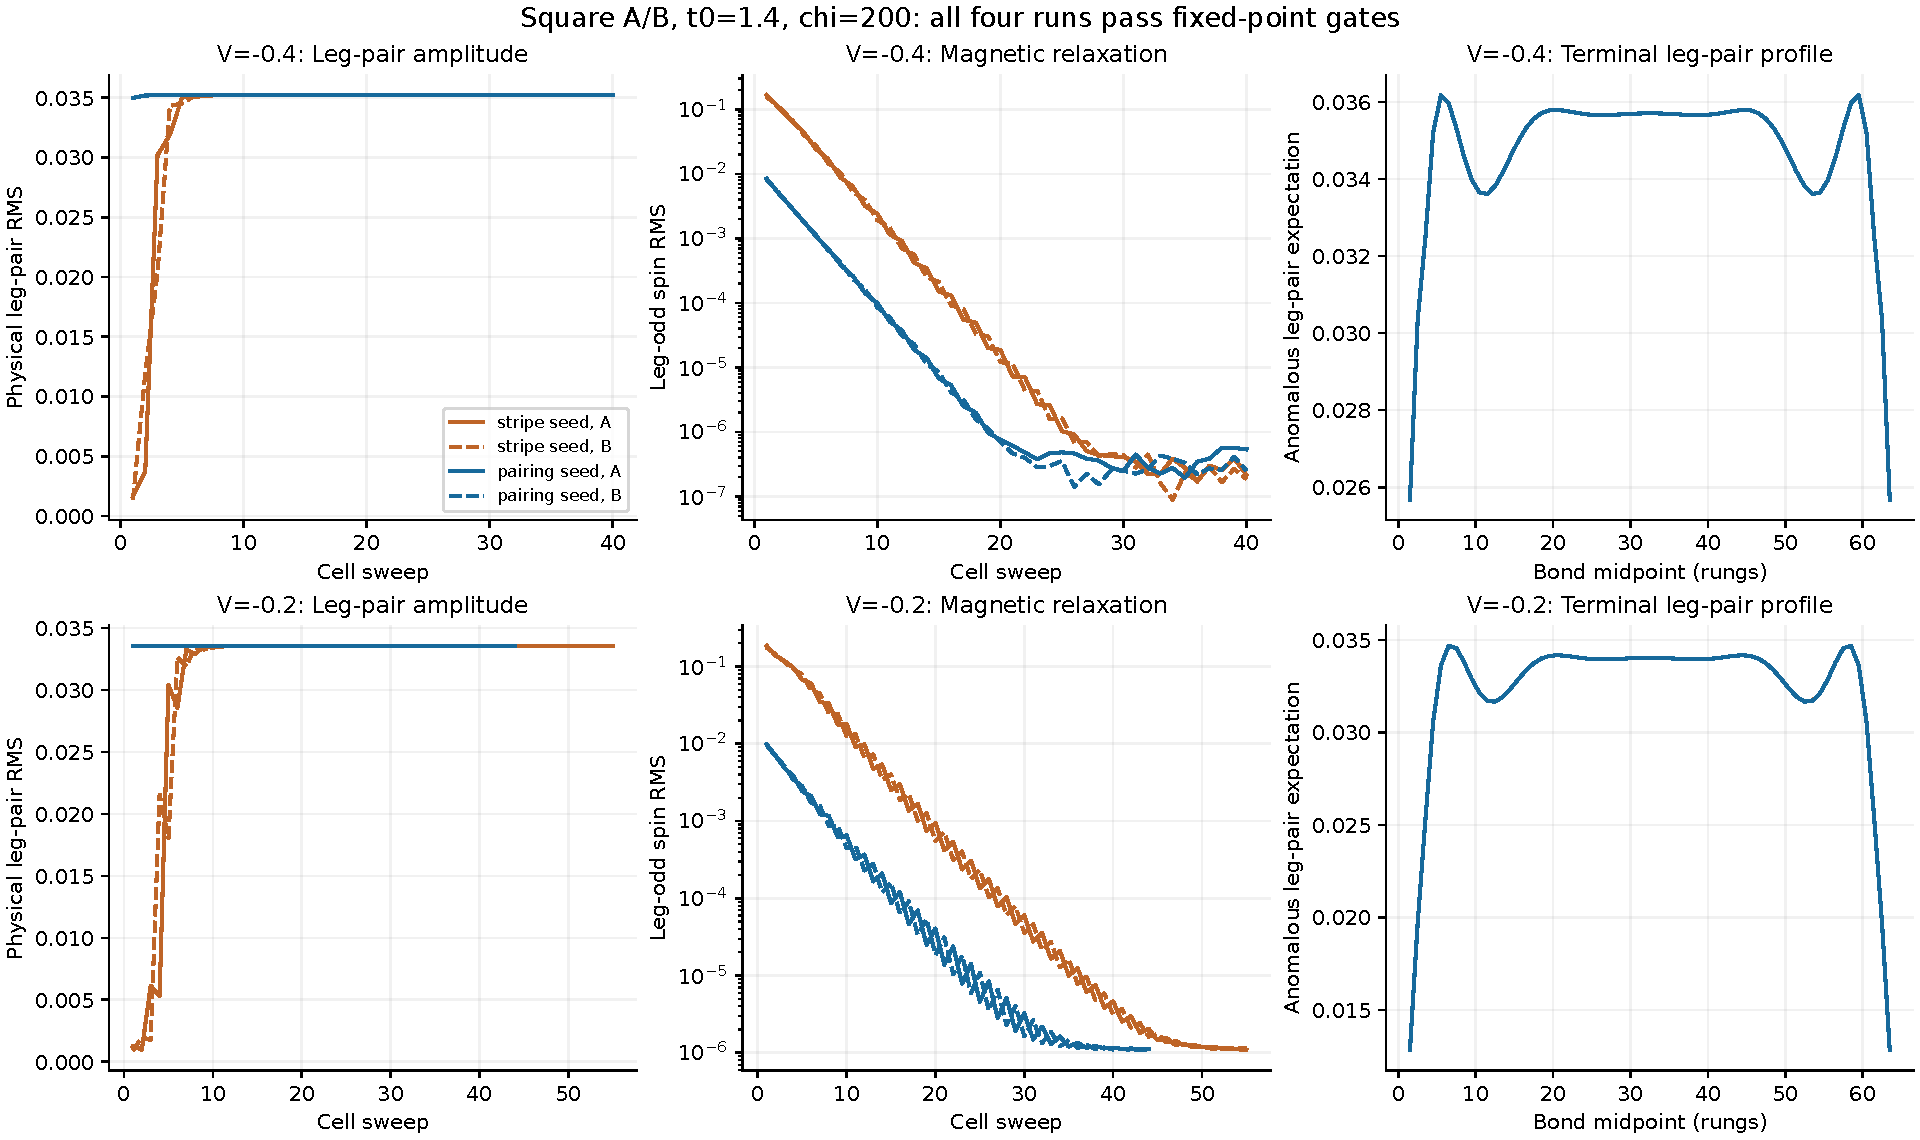
\includegraphics[width=\textwidth]{square_AB_complete.pdf}
\caption{Both square seeds lose their magnetic component and approach the
same paired solution at each attractive interaction. A/B curves nearly
coincide. Unlike the retrospective stripe endpoints, these four states
pass the stored stationarity gates.}
\end{figure}
\begin{figure}[p]\centering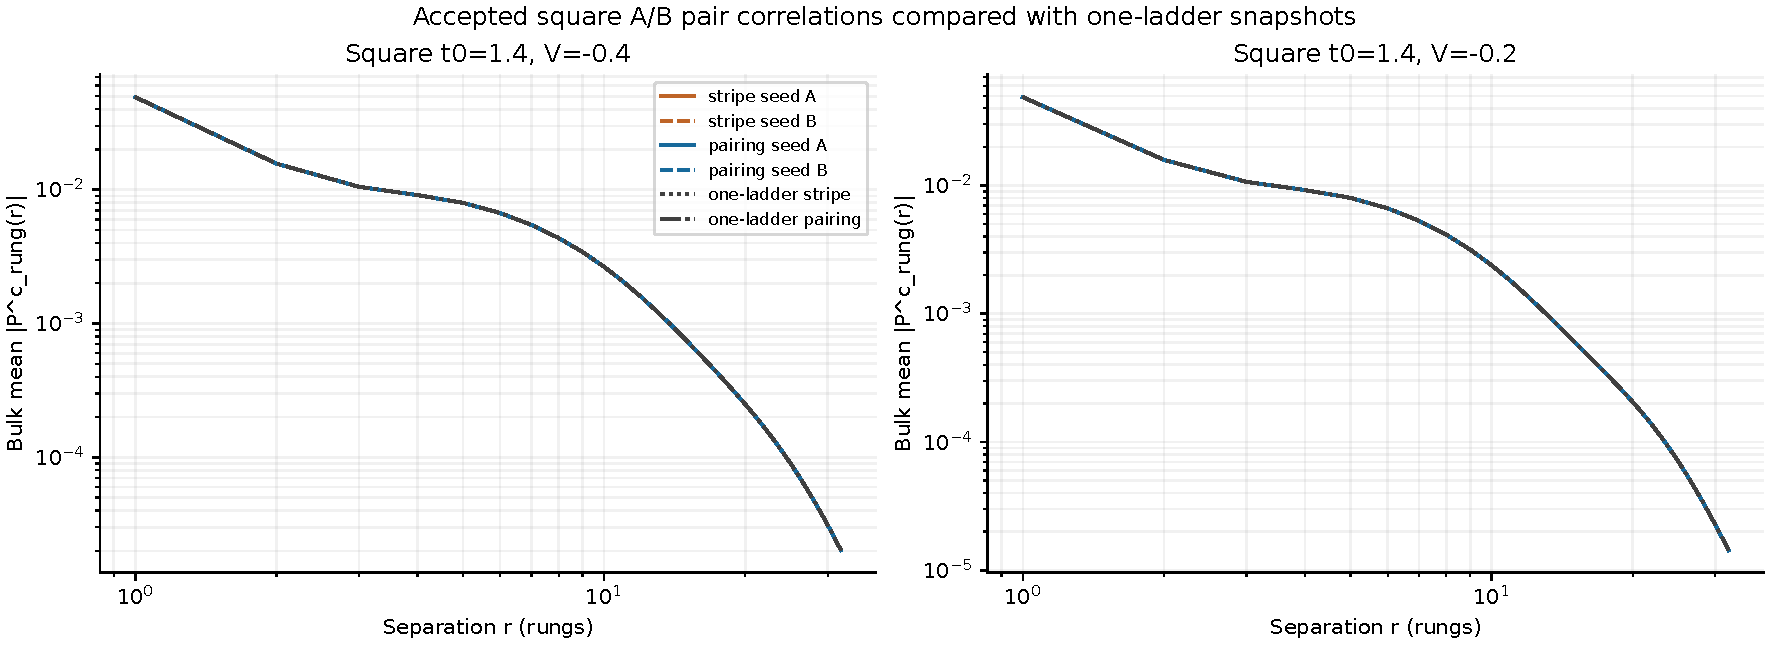
\includegraphics[width=\textwidth]{square_AB_pair_correlations.pdf}
\caption{Connected rung correlations in accepted square A/B states and
earlier one-ladder snapshots. Agreement supports the specific two-ladder
extension, without establishing stability against all transverse modes.}
\end{figure}
\clearpage

\section{Verification and reproducibility}
Run \texttt{python scripts/analyze\_pair\_correlations\_20260922.py} from
the ladder project. It reads synchronized artifacts and writes this report's
tables and vector/PDF and PNG figures. It never modifies states, manifests,
receipts, histories, acceptance flags or measurement files; it runs no DMRG.

The source audit checks 66 complete version-2 diagnostic files against
receipt hashes, full-source identifiers, compact-state hashes, model and
configuration provenance. It checks finite matrices, Hermiticity, the four
raw/connected Gram matrices' positive-semidefinite property to $10^{-9}$,
connected subtraction, within-class consistency and density/spin agreement
with saved states. All measured imaginary parts and connected-subtraction
residuals are zero in these real-state files. This establishes consistency
of the supplied measurements, not independent convergence in $L$ or $\chi$.

\begin{itemize}
\item \texttt{coverage.csv}: original branch indices and retry provenance.
\item \texttt{source\_validation.json}: source paths, hashes and matrix checks.
\item \texttt{correlation\_summary.csv}: all 66 coupled MPSs and the isolated reference.
\item \texttt{distance\_curves.csv}: full/connected signed and magnitude curves.
\item \texttt{reference\_window\_fits.csv}: every reference, direction and fit window.
\item \texttt{bulk\_cut\_sensitivity.csv}: alternate edge exclusions.
\item \texttt{stripe\_wall\_comparison.json}: both seeds and all striped trellis ladders.
\item \texttt{square\_AB\_results.json}: four endpoint gate and energy audits.
\end{itemize}

The physical conclusion is finite-distance survival of local pairing in
the measured stripes, together with suppressed long-distance propagation
and surviving rung/leg sign structure. The new accepted square results
strengthen the paired side of the comparison. Fully stationary stripes,
matched bond-dimension/length checks and dynamical or phase-response
observables are still required for stronger mechanism claims.
\end{document}
